\documentclass[11pt]{article}
\usepackage{graphicx,color,fullpage,url}
\usepackage{amsmath,amssymb}
\usepackage[font={small}]{caption}
\usepackage{natbib}
\bibliographystyle{abbrvnat}
\usepackage[nice]{nicefrac}

\usepackage[pdftex, pdftitle={My title}, pdflang={en-GB}]{hyperref}
\renewcommand{\familydefault}{\sfdefault}
%\usepackage{axessibility}
%\usepackage{accessibility}

% - fonts
%\usepackage{tgheros}
\usepackage{sansmathfonts}
\usepackage[scaled=0.95]{helvet}
\renewcommand{\rmdefault}{\sfdefault}

\title{Notes on the Numerical Methods in \texttt{pfsspy}}
\author{A. R. Yeates\\ Department of Mathematical Sciences, Durham University, UK}
\date{\today}

\newcommand{\file}[1]{\textcolor{blue}{\texttt{#1}}}
\newcommand{\flag}[1]{\textcolor{magenta}{\texttt{#1}}}

\renewcommand{\t}[1]{\texttt{#1}}
\renewcommand{\d}{\,\textrm{d}}
\newcommand{\dy}{\partial}

\newcommand{\dr}{\Delta_\rho}
\newcommand{\ds}{\Delta_s}
\newcommand{\dph}{\Delta_\phi}

\newcommand{\nr}{n_\rho}
\newcommand{\ns}{n_s}
\newcommand{\nph}{n_\phi}

\newcommand{\half}{\nicefrac{1}{2}}
\newcommand{\thr}{\nicefrac{3}{2}}

\newcommand{\Ab}{\boldsymbol{A}}
\newcommand{\Bb}{\boldsymbol{B}}
\newcommand{\Eb}{\boldsymbol{E}}
\newcommand{\Nb}{\boldsymbol{N}}
\newcommand{\eb}{\boldsymbol{e}}
\newcommand{\jb}{\boldsymbol{j}}
\newcommand{\nb}{\boldsymbol{n}}
\newcommand{\vb}{\boldsymbol{v}}

\newcommand{\ex}{\,\mathrm{e}}
\newcommand{\evr}{\,\mathrm{e}_\rho}
\newcommand{\evs}{\,\mathrm{e}_s}
\newcommand{\evp}{\,\mathrm{e}_\phi}
\newcommand{\evt}{\,\mathrm{e}_\theta}

\newcommand{\LA}{{\cal A}}
\newcommand{\OB}{{\cal B}}

% Remove paragraph indentation
\setlength{\parindent}{0pc}%
\setlength{\parskip}{\medskipamount}

\begin{document}
\maketitle

\section{Basic Equations}

The \texttt{pfsspy} code solves the for a magnetic field satisfying
\begin{align}
\nabla\times\Bb=0,\qquad
\nabla\cdot\Bb = 0
\end{align}
in a spherical shell $1 \leq r \leq R_{ss}$, given boundary conditions
\begin{align}
&B_r(\theta,\phi) = g(\theta,\phi) \quad \textrm{on} \quad r=1,\\
&B_\theta=B_\phi=0 \quad \textrm{on} \quad r=R_{ss}. \label{eqn:bc1}
\end{align}
The function $g(\theta,\phi)$ is specified by the user.

\section{Numerical Grid}

\begin{figure}
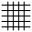
\includegraphics[width=\textwidth]{grid.jpg}
\caption{The numerical grid used in the solver.}
\label{fig:grid}
\end{figure}

The solver uses a rectilinear grid that is equally spaced in $\rho$, $s$, $\phi$, where
\[
\rho = \ln(r), \quad s=\cos\theta
\]
in terms of spherical coordinates $(r,\theta\,\phi)$. The coordinate scale factors $|\mathrm{d}\boldsymbol r/\mathrm{d}\rho|$, $|\mathrm{d}\boldsymbol r/\mathrm{d}s|$, $|\mathrm{d}\boldsymbol r/\mathrm{d}\phi|$ are
\[
h_\rho = r = \mathrm{e}^\rho,\quad h_s = \frac{r}{\sin\theta} = \frac{\mathrm{e}^\rho}{\sqrt{1-s^2}}, \quad h_\phi = r\sin\theta = \mathrm{e}^\rho\sqrt{1-s^2}.
\]
The grid is illustrated in Figure \ref{fig:grid}. Note that the longitudinal cell size goes to zero at the poles; these points are treated specially in the calculation of $\Bb$. Note also that, since $s$ is a decreasing function of $\theta$, the components of a vector $\boldsymbol{v}$ in $(\rho,s,\phi)$ are $v_\rho = v_r$ but $v_s = -v_\theta$.

We define the number of grid cells $\nr$, $\ns$, $\nph$, with corresponding uniform spacings
\[
\dr = \frac{\ln(R_{ss})}{\nr}, \quad \ds = \frac{2}{\ns}, \quad \dph = \frac{2\pi}{\nph}.
\]
Note that the boundaries in $s$ are at the poles $s=\pm1$, at which points $h_\phi$ is not defined. The solution is periodic in the longitudinal ($\phi$) direction.


\section{Numerical method}

\subsection{Overall strategy}

Rather than writing $\Bb = \nabla\chi$ and solving $\nabla^2\chi=0$, we write instead $\Ab = \nabla\times\big(\psi \evr\big)$. Then accounting for the unusual coordinates we get
\begin{align}
\Bb &=  \frac{1}{h_\rho h_sh_\phi}
\begin{vmatrix}
h_\rho\evr & h_\phi\evp & h_s\evs\\
\dy_\rho & \dy_\phi & \dy_s\\
0 & \frac{h_\phi}{h_s}\dy_s\psi & -\frac{h_s}{h_\phi}\dy_\phi\psi
\end{vmatrix}\\
&= -\frac{1}{h_sh_\phi}\left[\dy_s\left(\frac{h_\phi}{h_s}\dy_s\psi\right) + \dy_\phi\left(\frac{h_s}{h_\phi}\dy_\phi\psi\right) \right]\evr + \frac{1}{h_\rho h_\phi}\dy_\phi\dy_\rho\psi\evp + \frac{1}{h_\rho h_s}\dy_s\dy_\rho\psi\evs\\
&= -\Delta_\perp\psi\evr + \frac{1}{h_\phi}\dy_\phi\left(\frac{1}{h_\rho}\dy_\rho\psi\right)\evp + \frac{1}{h_s}\dy_s\left(\frac{1}{h_\rho}\dy_\rho\psi\right)\evs.
\end{align}
This will take the curl-free form $\Bb = \nabla\big(\tfrac1{h_\rho}\dy_\rho\psi\big)$ provided that
\begin{equation}
\nabla^2_\perp\psi = -\frac{1}{h_\rho}\dy_\rho\left(\frac{1}{h_\rho}\dy_\rho\psi\right),
\label{eqn:psi}
\end{equation}
so our strategy is to solve Equation \eqref{eqn:psi} for $\psi$, then reconstruct $\Ab$ and $\Bb$. The reason for doing it this way is that it allows us to compute $\Ab$ as well as $\Bb$ (again, for legacy reasons).

\subsection{Numerical solution}

We follow the method described in \cite{vanballe2000}, except that we modify the finite-difference discretisation to suit our particular coordinates.

The discretisation is chosen so that we will have $\nabla\times\Bb=0$ to machine precision on a staggered grid, when the curl is taken using central differences. This property of essentially zero current density is required when using the PFSS solution to, e.g., initialize non-potential simulations. It would not typically be achieved by interpolating a spherical harmonic solution onto the numerical grid. However, we will see that the discrete solution effectively computes discrete approximations of the spherical harmonics, tailored to our particular difference formula.

In the following subsections, we describe the numerical solution in more detail.

\subsubsection{Variables}

Let the coordinate grid points be defined by
\begin{align*}
&\rho^k = k\dr, \qquad k=0,\ldots, n_\rho,\\
&s^j = j\ds - 1, \qquad j=0,\ldots, n_s,\\
&\phi^i = i\dph, \qquad i=0,\ldots, n_\phi.
\end{align*}
\textcolor{blue}{In the code the first two arrays are called \texttt{rg} and \texttt{sg} (that for \texttt{pg} is not required). There are also arrays \texttt{rc},  \texttt{sc} and \texttt{pc} corresponding to the cell centres, i.e. $\rho^{k+1/2}$, $s^{j+1/2}$ and $\phi^{i+1/2}$.}

To deal with the curvilinear coordinates, we define the edge lengths
\begin{align*}
&L_\rho^{k+\half,j,i} = \int_{\rho^k}^{\rho^{k+1}} h_\rho\,\mathrm{d}\rho = \ex^{\rho^{k+1}} - \ex^{\rho^k},\\
&L_s^{k,j+\half,i} = \int_{s^j}^{s^{j+1}} h_s\,\mathrm{d}s = \ex^{\rho^k}\big(\arcsin(s^{j+1}) - \arcsin(s^j)\big),\\
&L_\phi^{k,j,i+\half} = \int_{\phi^i}^{\phi^{i+1}} h_\phi\,\mathrm{d}\phi = \ex^{\rho^k}\sigma^j\dph.
\end{align*}
Here we used the fact that $\dr$, $\ds$ and $\dph$ are constant, and used the shorthand
\[
\sigma^j := \sqrt{1 - (s^j)^2}.
\]
Similarly we define the areas of the cell faces
\begin{align*}
&S_\rho^{k,j+\half,i+\half} =  \int_{\phi^i}^{\phi^{i+1}}\int_{s^j}^{s^{j+1}} h_s h_\phi\,\mathrm{d}s\mathrm{d}\phi = \ex^{2\rho^k}\ds\dph,\\
&S_s^{k+\half,j,i+\half} = \int_{\rho^k}^{\rho^{k+1}}\int_{\phi^i}^{\phi^{i+1}} h_\rho h_\phi\,\mathrm{d}\phi\mathrm{d}\rho = \tfrac12\big(\ex^{2\rho^{k+1}} - \ex^{2\rho^{k}}\big)\sigma^j\,\dph,\\
&S_\phi^{k+\half,j+\half,i} = \int_{\rho^k}^{\rho^{k+1}}\int_{s^j}^{s^{j+1}}h_\rho h_s\,\mathrm{d}s\mathrm{d}\rho = \tfrac12\big(\ex^{2\rho^{k+1}}- \ex^{2\rho^k}\big)\big(\arcsin(s^{j+1}) - \arcsin(s^j)\big).
\end{align*}
\textcolor{blue}{In the code the face areas are stored in arrays \texttt{Sbr}, \texttt{Sbs} and \texttt{Sbp} (with only the dimensions required).}

In the code the magnetic field $\Bb$ is defined staggered on the face centres, so $B_\rho^{k,j+\half,i+\half}$, $B_s^{k+\half,j,i+\half}$, $B_\phi^{k+\half,j+\half,i}$. \textcolor{blue}{These variables are called \texttt{br}, \texttt{bs} and \texttt{bp}.}

The vector potential is located on the corresponding cell edges, so $A_\rho^{k+\half,j,i}$, $A_s^{k,j+\half,i+\half}$, $A_\phi^{k,j,i+\half}$. In fact, these values are never required on their own, only multiplied by the corresponding edge lengths. \textcolor{blue}{So the variables \texttt{alr}, \texttt{als} and \texttt{alp} correspond to the products $L_\rho A_\rho$, $L_sA_s$ and $L_\phi A_\phi$, respectively.}

Finally, the potential $\psi$ is located on the $\rho$-faces (like $B_\rho$), so $\psi^{k,j+\half,i+\half}$. \textcolor{blue}{It is stored in the variable \texttt{psi}.}

\subsubsection{Derivatives}

Firstly, we have $\Ab = \nabla\times\big(\psi\evr\big)$. Numerically, this is approximated by
\begin{equation}
A_s^{k,j+\half,i} = -\frac{\psi^{k,j+\half,i+\half} - \psi^{k,j+\half,i-\half}}{L_\phi^{k,j+\half,i}}, \qquad A_\phi^{k,j,i+\half} = \frac{\psi^{k,j+\half,i+\half} - \psi^{k,j-\half,i+\half}}{L_s^{k,j,i+\half}}.
\label{eqn:as}
\end{equation}
The magnetic field $\Bb = \nabla\times\Ab$ is then approximated by
\begin{align}
&(S_\rho B_\rho)^{k,j+\half,i+\half} = (L_s A_s)^{k,j+\half,i+1} - (L_s A_s)^{k,j+\half,i} - (L_\phi A_\phi)^{k,j+1,i+\half} + (L_\phi A_\phi)^{k,j,i+\half},\\
&(S_s B_s)^{k+\half,j,i+\half} = (L_\phi A_\phi)^{k+1,j,i+\half} - (L_\phi A_\phi)^{k,j,i+\half},\\
&(S_\phi B_\phi)^{k+\half,j+\half,i} =  - (L_s A_s)^{k+1,j+\half,i} + (L_s A_s)^{k,j+\half,i}. \label{eqn:bp}
\end{align}
These formulae correspond to Stokes' Theorem applied to the cell face.
The condition $\nabla\times\Bb=0$ may be expressed similarly as
\begin{align}
&0 = (L_s B_s)^{k+\half,j,i-\half} - (L_s B_s)^{k+\half,j,i+\half} - (L_\phi B_\phi)^{k+\half,j+\half,i} + (L_\phi B_\phi)^{k+\half,j-\half,i},\label{eqn:j1}\\
&0 = (L_\phi B_\phi)^{k+\half,j+\half,i} - (L_\phi B_\phi)^{k-\half,j+\half,i} - (L_\rho B_\rho)^{k,j+\half,i+\half} + (L_\rho B_\rho)^{k,j+\half,i-\half},\label{eqn:j2}\\
&0 = (L_\rho B_\rho)^{k,j+\half,i+\half} - (L_\rho B_\rho)^{k,j-\half,i+\half} - (L_s B_s)^{k+\half,j,i+\half} + (L_s B_s)^{k-\half,j,i+\half}.\label{eqn:j3}
\end{align}
Note that the factors $L_\rho$, $L_s$, $L_\phi$ here are defined normal to the cell faces, not on the edges. But they have the same formulae.

In fact, condition \eqref{eqn:j1} is automatically satisfied. This may be shown using equations \eqref{eqn:as} to \eqref{eqn:bp}, together with our formulae for $L_s$, $L_\phi$, $S_s$ and $S_\phi$.

Below, we will discretise \eqref{eqn:psi} in such a way that conditions \eqref{eqn:j2} and \eqref{eqn:j3} are also satisfied exactly (up to rounding error).

\subsubsection{Boundary conditions for $\Bb$}

Boundary conditions are needed when \texttt{br}, \texttt{bs}, \texttt{bp} are averaged to the grid points for output. We use a layer of ``ghost cells'', whose values are set by the following boundary conditions:
\begin{enumerate}
\item In $\phi$, \texttt{br} and \texttt{bs} are simply periodic.
\item At the outer boundary $\rho=\log(R_{ss})$, ghost values of \texttt{bs} and \texttt{bp} are set assuming constant gradient in $\rho$.
\item At the inner boundary, $\rho=0$, ghost values of \texttt{bs} and \texttt{bp} are set using equations \eqref{eqn:j2} and \eqref{eqn:j3} (effectively assuming zero horizontal current density).
\item At the polar boundaries, the ghost value of \texttt{br} is set to the polemost interior value from the opposite side of the grid. Similarly, \texttt{bp} is set to minus the polemost interior value from the opposite side of the grid. The values of \texttt{bs} at the poles are not meaningful as the cell faces have zero area. However, they are set to the average of the two neighbouring interior values at that longitude (with the opposite one being reversed in sign).
\end{enumerate}
Some of these conditions are chosen for compatibility with other codes, and are not necessarily the most straightforward option for a pure PFSS solver.

\subsubsection{Discretization of Equation \eqref{eqn:psi}}

First, we approximate the two-dimensional Laplacian $\nabla^2_\perp\psi$ by
\begin{align*}
&\nabla^2_\perp\psi^{k,j+\half,i+\half} = \frac{1}{S_\rho^{k,j+\half,i+\half}}\left[
\frac{L_s^{k,j+\half,i+1}}{L_\phi^{k,j+\half,i+1}}\big(\psi^{k,j+\half,i+\thr} - \psi^{k,j+\half,i+\half}\big) -
\frac{L_s^{k,j+\half,i}}{L_\phi^{k,j+\half,i}}\big(\psi^{k,j+\half,i+\half} - \psi^{k,j+\half,i-\half}\big) \right.\nonumber\\
&\left. +
 \frac{L_\phi^{k,j+1,i+\half}}{L_s^{k,j+1,i+\half}}\big(\psi^{k,j+\thr,i+\half} - \psi^{k,j+\half,i+\half}\big) - \frac{L_\phi^{k,j,i+\half}}{L_s^{k,j,i+\half}}\big(\psi^{k,j+\half,i+\half} - \psi^{k,j-\half,i+\half}\big)
 \right]
\end{align*}
As shorthand we define the quantities
\[
U^{j+\half} = \left(\frac{L_s}{\ds\dph L_\phi}\right)^{j+\half}, \qquad V^j = \left(\frac{L_\phi}{\ds\dph L_s}\right)^j,
\]
noting that these both depend on $j$ only. \textcolor{blue}{In the code these are called \texttt{Uc} and \texttt{Vg}.} Then we can write our discretization as
\begin{align}
\nabla^2_\perp\psi^{k,j+\half,i+\half}  = \frac{1}{\ex^{2\rho^k}}\Big[U^{j+\half}\big(\psi^{k,j+\half,i+\thr} - \psi^{k,j+\half,i-\half} \big) + V^{j+1}\psi^{k,j+\thr,i+\half} + V^{j}\psi^{k,j-\half,i+\half}\nonumber\\
 - \Big(2U^{j+\half} + V^{j+1} + V^{j}\Big)\psi^{k,j+\half,i+\half}\Big].
 \label{eqn:lapl}
\end{align}
This is the left-hand side of \eqref{eqn:psi}.

To discretize the right-hand side of \eqref{eqn:psi}, we use the approximation
\begin{align}
-\frac{1}{h_\rho}\dy_\rho\left(\frac{1}{h_\rho}\dy_\rho\psi\right)^{k,j+\half,i+\half} = -\frac{c(\dr)}{L_\rho^{k,j+\half,i+\half}}\left(\frac{\psi^{k+1,j+\half,i+\half} - \psi^{k,j+\half,i+\half}}{L_\rho^{k+\half,j+\half,i+\half}} - \frac{\psi^{k,j+\half,i+\half} - \psi^{k-1,j+\half,i+\half}}{L_\rho^{k-\half,j+\half,i+\half}} \right),
\end{align}
where
\[
c(\dr) = \frac{2\ex^{\dr/2}}{\ex^{\dr} + 1} = \mathrm{sech}\left(\frac{\dr}{2}\right).
\]
Combining this with \eqref{eqn:lapl}, we arrive at
\begin{align}
U^{j+\half}\big(\psi^{k,j+\half,i+\thr} - \psi^{k,j+\half,i-\half} \big) + V^{j+1}\psi^{k,j+\thr,i+\half} + V^{j}\psi^{k,j-\half,i+\half}
 - \Big(2U^{j+\half} + V^{j+1} + V^{j}\Big)\psi^{k,j+\half,i+\half}\nonumber\\
 = -\frac{c(\dr)\ex^{2\rho^k}}{L_\rho^{k,j+\half,i+\half}}\left(\frac{\psi^{k+1,j+\half,i+\half} - \psi^{k,j+\half,i+\half}}{L_\rho^{k+\half,j+\half,i+\half}} - \frac{\psi^{k,j+\half,i+\half} - \psi^{k-1,j+\half,i+\half}}{L_\rho^{k-\half,j+\half,i+\half}} \right).
 \label{eqn:main}
\end{align}
The reader may verify algebraically that conditions \eqref{eqn:j2} and \eqref{eqn:j3} follow if this finite-difference equation is satisfied.

\subsubsection{Method of solution}

Equation \eqref{eqn:main}, together with the appropriate boundary conditions, yields a large (but sparse) system of $\nr\ns\nph\times \nr\ns\nph$ linear equations to solve. Fortunately, following \cite{vanballe2000}, we can reduce this to a series of symmetric tridiagonal eigenvalue problems, if we look for eigenfunctions of the form
\begin{equation}
\psi^{k,j+\half,i+\half} = f^kQ_{lm}^{j+\half}\,\ex^{2\pi I mi/\nph}.
\label{eqn:eig}
\end{equation}
Here the $k$ in $f^k$ is a power, not an index, and $I$ is the square root of $-1$ (since we already used $i$ and $j$ for indices). This reduction will enable very efficient solution of the linear system.

Substituting \eqref{eqn:eig} in Equation \eqref{eqn:main} gives
\begin{align}
-V^{j}Q^{j-\half}_{lm} + \left(V^{j} + V^{j+1}+ 4U^{j+\half}\sin^2\left(\tfrac{\pi m}{\nph}\right) \right)Q^{j+\half}_{lm} - V^{j+1}Q^{j+\thr}_{lm} \nonumber\\
= \frac{c(\dr)\mathrm{e}^{2\rho^k}}{L_\rho^{k,j+\half,i+\half}}\left(\frac{f - 1}{L_\rho^{k+\half,j+\half,i+\half}} - \frac{1 - f^{-1}}{L_\rho^{k-\half,j+\half,i+\half}} \right)Q_{lm}^{j+\half}.
\end{align}
The right-hand side can be simplified since the dependence on $k$ cancels out. This leaves the tridiagonal eigenvalue problem
\begin{equation}
-V^{j}Q^{j-\half}_{lm} + \left(V^{j} + V^{j+1}+ 4U^{j+\half}\sin^2\left(\tfrac{\pi m}{\nph}\right) \right)Q^{j+\half}_{lm} - V^{j+1}Q^{j+\thr}_{lm} = \lambda_{lm}Q_{lm}^{j+\half},
\end{equation}
where $f$ is determined from the eigenvalues $\lambda_{lm}$ by solving the quadratic relation
\begin{equation}
\lambda_{lm} = \frac{c(\dr)}{\mathrm{e}^{\dr/2} - \mathrm{e}^{-\dr/2}} \left(\frac{1-f^{-1}}{1-\mathrm{e}^{-\dr}} - \frac{f-1}{\mathrm{e}^{\dr} - 1}\right).
\end{equation}
This may be rearranged into the form
\begin{equation}
f^2 - \left[1 + \mathrm{e}^{\dr} + \mathrm{sech}\left(\frac{\dr}{2}\right)\lambda_{lm}(\mathrm{e}^{\dr}-1)(\mathrm{e}^{\dr/2} - \mathrm{e}^{-\dr/2}) \right]f + \mathrm{e}^{\dr} = 0,
\end{equation}
with two solutions for each $l$, $m$ given by
\begin{equation}
f_{lm}^+, f_{lm}^- = F_{lm} \pm \sqrt{F_{lm}^2 - \mathrm{e}^{\dr}}, \quad \textrm{where} \quad F_{lm} = \tfrac12\Big[1 + \mathrm{e}^{\dr} + \lambda_{lm}(\mathrm{e}^{\dr}-1)\sinh(\dr) \Big].
\end{equation}
\textcolor{blue}{In the code, the eigenvalues are called \texttt{lam} and the corresponding matrix of eigenvectors is \texttt{Q}. The solutions $f_{lm}^+$ and $f_{lm}^-$ are called \texttt{ffp} and \texttt{ffm} respectively.}

The solution may then be written as a sum of these two sets of radial eigenfunctions:
\begin{equation}
\psi^{k,j+\half,i+\half} = \sum_{l=0}^{\ns-1}\sum_{m=0}^{\nph-1}\Big[c_{lm}(f_{lm}^+)^k + d_{lm}(f_{lm}^-)^k) \Big] Q_{lm}^{j+\half}\ex^{2\pi I mi/\nph}.
\label{eqn:psisum}
\end{equation}
The coefficients $c_{lm}$ and $d_{lm}$ are then determined by the radial boundary conditions:
\begin{enumerate}
\item At the inner boundary $\rho = 0$, where $k=0$, we want  $B_\rho = -\nabla^2_\perp\psi$ to match our given distribution $g^{j+\half,i+\half}$.
We have
\[
B_\rho^{k,j+\half,i+\half} = \sum_{l=0}^{\ns-1}\sum_{m=0}^{\nph-1}\frac{\lambda_{lm}}{\mathrm{e}^{2\rho^k}}\Big[c_{lm}(f_{lm}^+)^k + d_{lm}(f_{lm}^-)^k) \Big] Q_{lm}^{j+\half}\mathrm{e}^{2\pi I mi/\nph},
\]
so
\[
g^{j+\half,i+\half} = \sum_{l=0}^{\ns-1}\sum_{m=0}^{\nph-1}\frac{\lambda_{lm}}{\mathrm{e}^{2\rho^0}}\Big[c_{lm} + d_{lm}\Big] Q_{lm}^{j+\half}\mathrm{e}^{2\pi I mi/\nph}.
\]
We take the discrete Fourier transform of $g^{j+\half,i+\half}$ in $i$, so that (noting $\ex^{\rho^0}=1$),
\[
\sum_{l=0}^{\ns-1}\sum_{m=0}^{\nph-1}\lambda_{lm}
\Big[c_{lm} + d_{lm}\Big] Q_{lm}^{j+\half}\,\mathrm{e}^{2\pi I mi/\nph} = \sum_{m=0}^{\nph-1}b_m^{j+\half}\,\mathrm{e}^{2\pi I mi/\nph}.
\]
Then the orthonormality of $Q_{lm}^{j+\half}$ for different $l$ allows us to determine
\begin{equation}
c_{lm} + d_{lm} = \frac{1}{\lambda_{lm}}\sum_{j=0}^{\ns-1}b_m^{j+\half}Q_{lm}^{j+\half}.
\label{eqn:dc2}
\end{equation}
\item At the source (outer) surface $\rho=\ln(R_{ss})$, where $k=\nr$, there are two options.
\begin{enumerate}
\item  \emph{Radial field.} We impose $\dy_\rho\psi = 0$, in the form $\psi^{\nr,j+\half,i+\half}=\psi^{\nr-1,j+\half,i+\half}$, which gives
\begin{equation}
\frac{d_{lm}}{c_{lm}} = \frac{(f_{lm}^+)^{\nr} - (f_{lm}^+)^{\nr-1}}{(f_{lm}^-)^{\nr-1} - (f_{lm}^-)^{\nr}}.
\label{eqn:dc1}
\end{equation}
(Numerically it is better to compute this ratio the other way up, to prevent overflow.)
\item  \emph{Imposed $B_r$.} In this case the boundary condition is treated similarly to the inner boundary. We require
\[
\hat{g}^{j+\half,i+\half} = \sum_{l=0}^{\ns-1}\sum_{m=0}^{\nph-1}\frac{\lambda_{lm}}{\mathrm{e}^{2\rho^{n_\rho}}}\Big[c_{lm}(f_{lm}^+)^{n_\rho} + d_{lm}(f_{lm}^-)^{n_\rho}\Big] Q_{lm}^{j+\half}\mathrm{e}^{2\pi I mi/\nph},
\]
so we may again take the discrete Fourier transform to end up with
\begin{equation}
c_{lm}(f_{lm}^+)^{n_\rho} + d_{lm}(f_{lm}^-)^{n_\rho} = \frac{\mathrm{e}^{2\rho^{n_\rho}}}{\lambda_{lm}}\sum_{j=0}^{\ns-1}\hat{b}_m^{j+\half}Q_{lm}^{j+\half},
\label{eqn:dc3}
\end{equation}
\end{enumerate}
\end{enumerate}
Solving \eqref{eqn:dc1} simultaneously with either \eqref{eqn:dc2} or \eqref{eqn:dc3} gives $c_{lm}$ and $d_{lm}$. \textcolor{blue}{These are called \texttt{clm} and \texttt{dlm} in the code.}

Remark: as we increase the grid resolution, the eigenfunctions $Q_{lm}^{j+\half}$, which are functions of $\theta$, should converge to the corresponding associated Legendre polynomials $P_l^m(\cos\theta)$, up to normalization. This is illustrated in Figure \ref{fig:Q}.

\begin{figure}
\centering
\includegraphics[width=0.7\textwidth]{Q.png}
\caption{Comparison of $P_l^m(\cos\theta)$ (coloured lines) with the discrete eigenfunctions $Q_{lm}^{j+\half}$ (black dots), for $m=6$ and $l=0,\ldots,4$, at resolution $\ns=60$ and $\nph=120$. \label{fig:Q}}
\end{figure}


\bibliography{refs}

\end{document}
